\subsection{SPI-Master}
\label{sec:SPIMaster}

The microcontroller have to share information with the FPGA, and according to the requirements mentioned in section \ref{sec:Primaryrequirements}, this communication has to happen using Serial Peripheral Interface (SPI). The protocol will operate as descriped in section \ref{sec:SPIcommunication}. It is therefore important that this link never will be a bottleneck for the system application. 

The requirements of the minimum bit-rate depends om what data that needs to be send, and how often it needs to send it. Since the PID-controller is placed in the FPGA, the application only needs to update the current position once every 5 ms, which is the minimal delay that freeRTOS can put on a task. 

The length of the messages send is defined by the driver placed in the FPGA. As described in section \ref{sec:Implementation} all messages will have the length of 14 bits. Updating both pan and tilt requires two messages. Concidering all other messeges but the main pulling sequence neglecteble relult in a total bitrate of:

\begin{equation}
Bitrate = \frac{
14 bit * 2	
}{
0.05s
} = 5.600 bit/sec 
\end{equation}

The Cortex M4 have a build in frescale spi module, that supports four different variations of spi, se appendix \ref{sec:CortexM4Datasheet}. However, by implementing the spi from scratch, it will give highest degree of control over the process, which is prefer in this project. 

% full dreasd task diagram
\begin{figure}
	\centering
	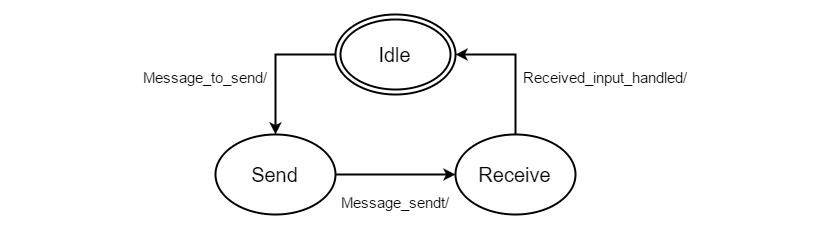
\includegraphics[scale = 0.7] {Billeder/SPI-master}
	\caption{The SPI-master state machine}
	\label{fig:SPI-master}
\end{figure}

The state machine for the task is illustrated in figure \ref{fig:SPI-master} is as simple at is gonna get. It consists of three states and is initiated waiting for a message to transmit from the spi\_tx\_queue. When a message is pulled from the queue it jumps to the send state, and after sending the message, the received message will be handled by the P\&T API in the Receive task. From here it will only switch back to the idle state if the API call was successful, else it will continue till it succeeds. 

Mesure the performance 
 

 



